% !BIB TS-program = biber

\RequirePackage[l2tabu,orthodox]{nag}

\documentclass[headsepline,footsepline,footinclude=false,oneside,fontsize=11pt,paper=a4,listof=totoc,bibliography=totoc]{scrbook} % one-sided

% TODO: change citation style in settings
\PassOptionsToPackage{table,svgnames,dvipsnames}{xcolor}

\usepackage[utf8]{inputenc}
\usepackage[T1]{fontenc}
\usepackage[sc]{mathpazo}
\usepackage[ngerman,american]{babel}
\usepackage[autostyle]{csquotes}
\usepackage[%
  backend=biber,
  url=false,
  style=alphabetic,
  maxnames=4,
  minnames=3,
  maxbibnames=99,
  giveninits,
  uniquename=init]{biblatex} % TODO: adapt citation style
\usepackage{graphicx}
\usepackage{scrhack} % necessary for listings package
\usepackage{listings}
\usepackage{lstautogobble}
\usepackage{tikz}
\usepackage{pgfplots}
\usepackage{pgfplotstable}
\usepackage{booktabs}
\usepackage[final]{microtype}
\usepackage{caption}
\usepackage[printonlyused]{acronym}
\usepackage[hidelinks]{hyperref} % hidelinks removes colored boxes around references and links
\AtBeginDocument{%
	\hypersetup{
		pdftitle=\getTitle,
		pdfauthor=\getAuthor,
	}
}
\usepackage{ifthen}

% for fachschaft_print.pdf
\makeatletter
\if@twoside
	\typeout{TUM-Dev LaTeX-Thesis-Template: twoside}
\else
	\typeout{TUM-Dev LaTeX-Thesis-Template: oneside}
\fi
\makeatother

\addto\extrasamerican{
	\def\lstnumberautorefname{Line}
	\def\chapterautorefname{Chapter}
	\def\sectionautorefname{Section}
	\def\subsectionautorefname{Subsection}
	\def\subsubsectionautorefname{Subsubsection}
}

\addto\extrasngerman{
	\def\lstnumberautorefname{Zeile}
}

% Themes
\ifthenelse{\equal{\detokenize{dark}}{\jobname}}{%
  % Dark theme
  \newcommand{\bg}{black} % background
  \newcommand{\fg}{white} % foreground
  \usepackage[pagecolor=\bg]{pagecolor}
  \color{\fg}
}{%
  % Light theme
  \newcommand{\bg}{white} % background
  \newcommand{\fg}{black} % foreground
}

\bibliography{bibliography}

\setkomafont{disposition}{\normalfont\bfseries} % use serif font for headings
\linespread{1.05} % adjust line spread for mathpazo font

% Add table of contents to PDF bookmarks
\BeforeTOCHead[toc]{{\cleardoublepage\pdfbookmark[0]{\contentsname}{toc}}}

% Define TUM corporate design colors
% Taken from http://portal.mytum.de/corporatedesign/index_print/vorlagen/index_farben
\definecolor{TUMBlue}{HTML}{0065BD}
\definecolor{TUMSecondaryBlue}{HTML}{005293}
\definecolor{TUMSecondaryBlue2}{HTML}{003359}
\definecolor{TUMBlack}{HTML}{000000}
\definecolor{TUMWhite}{HTML}{FFFFFF}
\definecolor{TUMDarkGray}{HTML}{333333}
\definecolor{TUMGray}{HTML}{808080}
\definecolor{TUMLightGray}{HTML}{CCCCC6}
\definecolor{TUMAccentGray}{HTML}{DAD7CB}
\definecolor{TUMAccentOrange}{HTML}{E37222}
\definecolor{TUMAccentGreen}{HTML}{A2AD00}
\definecolor{TUMAccentLightBlue}{HTML}{98C6EA}
\definecolor{TUMAccentBlue}{HTML}{64A0C8}

% Settings for pgfplots
\pgfplotsset{compat=newest}
\pgfplotsset{
  % For available color names, see http://www.latextemplates.com/svgnames-colors
  cycle list={TUMBlue\\TUMAccentOrange\\TUMAccentGreen\\TUMSecondaryBlue2\\TUMDarkGray\\},
}

% Settings for lstlistings
\lstset{%
  basicstyle=\ttfamily,
  columns=fullflexible,
  autogobble,
  keywordstyle=\bfseries\color{TUMBlue},
  stringstyle=\color{TUMAccentGreen},
  captionpos=b
}

%


\newcommand*{\getUniversity}{Technische Universität München}
\newcommand*{\getFaculty}{Informatics}
\newcommand*{\getDegree}{Informatics}
\newcommand*{\getSchool}{Computation, Information and Technology}
\newcommand*{\getTitle}{Seamless Synergy: Unifying Local Development and Cloud Execution in Machine Learning DevOps}
\newcommand*{\getTitleGer}{Nahtlose Synergie: Vereinheitlichung von lokaler Entwicklung und Cloud-Ausführung in DevOps für maschinelles Lernen}
\newcommand*{\getAuthor}{Baraa Alnassan}
\newcommand*{\getDoctype}{Bachelor's Thesis}
\newcommand*{\getSupervisor}{Jens Großklags}
\newcommand*{\getAdvisor}{Derui Zhu (TUM), Kaio Giurizatto Utsch (IT4IPM)}
\newcommand*{\getSubmissionDate}{September 1st 2024}
\newcommand*{\getSubmissionLocation}{Munich}

\begin{document}

% Set page numbering to avoid "destination with the same identifier has been already used" warning for cover page.
% (see https://en.wikibooks.org/wiki/LaTeX/Hyperlinks#Problems_with_Links_and_Pages).
\pagenumbering{alph}
\begin{titlepage}
  % HACK for two-sided documents: ignore binding correction for cover page.
  % Adapted from Markus Kohm's KOMA-Script titlepage=firstiscover handling.
  % See http://mirrors.ctan.org/macros/latex/contrib/koma-script/scrkernel-title.dtx,
  % \maketitle macro.
  \oddsidemargin=\evensidemargin\relax
  \textwidth=\dimexpr\paperwidth-2\evensidemargin-2in\relax
  \hsize=\textwidth\relax

  \centering

  \IfFileExists{logos/tum-\fg.pdf}{%
    \includegraphics[height=20mm]{logos/tum-\fg.pdf}
  }{%
    \vspace*{20mm}
  }

  \vspace{5mm}
  {\huge\MakeUppercase{School of \getSchool{} --- \getFaculty{}} \par}

  \vspace{5mm}
  {\large\MakeUppercase{\getUniversity{}} \par}

  \vspace{15mm}
  {\Large \getDoctype{} in \getDegree{} \par}

  \vspace{10mm}
  {\huge\bfseries \getTitle{} \par}

  \vspace{10mm}
  {\LARGE \getAuthor{}}

  \IfFileExists{logos/faculty-\fg.pdf}{%
    \vfill{}
    \includegraphics[height=20mm]{logos/faculty-\fg.pdf}
  }{}
\end{titlepage}


\frontmatter{}

\begin{titlepage}
  \centering

  \IfFileExists{logos/tum-\fg.pdf}{%
    \includegraphics[height=20mm]{logos/tum-\fg.pdf}
  }{%
    \vspace*{20mm}
  }

  \vspace{5mm}
  {\huge\MakeUppercase{School of \getSchool{} --- \getFaculty{}} \par}

  \vspace{5mm}
  {\large\MakeUppercase{\getUniversity{}} \par}

  \vspace{20mm}
  {\Large \getDoctype{} in \getDegree{} \par}

  \vspace{15mm}
  {\huge\bfseries \getTitle{} \par}

  \vspace{10mm}
  {\huge\bfseries \foreignlanguage{ngerman}{\getTitleGer{}} \par}

  \vspace{15mm}
  \begin{tabular}{l l}
    Author:          & \getAuthor{}         \\
    Supervisor:      & \getSupervisor{}     \\
    Advisor:         & \getAdvisor{}        \\
    Submission Date: & \getSubmissionDate{} \\
  \end{tabular}

  \IfFileExists{logos/faculty-\fg.pdf}{%
    \vfill{}
    \includegraphics[height=20mm]{logos/faculty-\fg.pdf}
  }{}
\end{titlepage}

\thispagestyle{empty}
\vspace*{0.8\textheight}
\noindent
I confirm that this \MakeLowercase{\getDoctype{}} is my own work and I have documented all sources and material used.

\vspace{15mm}
\noindent
\getSubmissionLocation{}, \getSubmissionDate{} \hspace{\fill} \getAuthor{}

\cleardoublepage{}

\addcontentsline{toc}{chapter}{Acknowledgments}
\thispagestyle{empty}

\vspace*{20mm}

\begin{center}
    {\usekomafont{sectioning}\usekomafont{section} Acknowledgments}
\end{center}

\vspace{10mm}

%TODO: Acknowledgments

\cleardoublepage{}

\chapter{\abstractname}

%TODO: Abstract

\microtypesetup{protrusion=false}
\tableofcontents{}
\microtypesetup{protrusion=true}

\mainmatter{}

% !TeX root = ../main.tex
% Add the above to each chapter to make compiling the PDF easier in some editors.

\chapter{Introduction}\label{chapter:introduction}

\section{Section}
Citation test~\parencite{latex}.

Acronyms must be added in \texttt{main.tex} and are referenced using macros. The first occurrence is automatically replaced with the long version of the acronym, while all subsequent usages use the abbreviation.

E.g. \texttt{\textbackslash ac\{TUM\}, \textbackslash ac\{TUM\}} $\Rightarrow$ \ac{TUM}, \ac{TUM}

For more details, see the documentation of the \texttt{acronym} package\footnote{\url{https://ctan.org/pkg/acronym}}.
\subsection{Subsection}

See~\autoref{tab:sample}, \autoref{fig:sample-drawing}, \autoref{fig:sample-plot}, \autoref{fig:sample-listing}.

\begin{table}[htpb]
  \caption[Example table]{An example for a simple table.}\label{tab:sample}
  \centering
  \begin{tabular}{l l l l}
    \toprule
      A & B & C & D \\
    \midrule
      1 & 2 & 1 & 2 \\
      2 & 3 & 2 & 3 \\
    \bottomrule
  \end{tabular}
\end{table}

\begin{figure}[htpb]
  \centering
  % This should probably go into a file in figures/
  \begin{tikzpicture}[node distance=3cm]
    \node (R0) {$R_1$};
    \node (R1) [right of=R0] {$R_2$};
    \node (R2) [below of=R1] {$R_4$};
    \node (R3) [below of=R0] {$R_3$};
    \node (R4) [right of=R1] {$R_5$};

    \path[every node]
      (R0) edge (R1)
      (R0) edge (R3)
      (R3) edge (R2)
      (R2) edge (R1)
      (R1) edge (R4);
  \end{tikzpicture}
  \caption[Example drawing]{An example for a simple drawing.}\label{fig:sample-drawing}
\end{figure}

\begin{figure}[htpb]
  \centering

  \pgfplotstableset{col sep=&, row sep=\\}
  % This should probably go into a file in data/
  \pgfplotstableread{
    a & b    \\
    1 & 1000 \\
    2 & 1500 \\
    3 & 1600 \\
  }\exampleA
  \pgfplotstableread{
    a & b    \\
    1 & 1200 \\
    2 & 800 \\
    3 & 1400 \\
  }\exampleB
  % This should probably go into a file in figures/
  \begin{tikzpicture}
    \begin{axis}[
        ymin=0,
        legend style={legend pos=south east},
        grid,
        thick,
        ylabel=Y,
        xlabel=X
      ]
      \addplot table[x=a, y=b]{\exampleA};
      \addlegendentry{Example A};
      \addplot table[x=a, y=b]{\exampleB};
      \addlegendentry{Example B};
    \end{axis}
  \end{tikzpicture}
  \caption[Example plot]{An example for a simple plot.}\label{fig:sample-plot}
\end{figure}

\begin{figure}[htpb]
  \centering
  \begin{tabular}{c}
  \begin{lstlisting}[language=SQL]
    SELECT * FROM tbl WHERE tbl.str = "str"
  \end{lstlisting}
  \end{tabular}
  \caption[Example listing]{An example for a source code listing.}\label{fig:sample-listing}
\end{figure}

\chapter{Background}\label{chapter:background}

Before diving into the details of the main objective of the thesis, it is important to understand some background knowledge. In this chapter i will introduce some necessary detailed background of the rise of \ac{ML}, and how the concenpt of \ac{MLOps} came to be.

\section{The Rise of Machine Learning}
\subsection{The Birth of Machine Learning (1950s)}
The foundations of machine learning were laid in the 1950s by computer scientists and mathematicians who sought to develop algorithms that could enable computers to learn from data \cite{MLHistory, Rahal2024, MLRise}. During this era, several key milestones shaped the field. Such as the Perceptron Algorithm - one of the earliest breakthroughs in machine learning - by Frank Rosenblatt \cite{Frank_Rosenblatt},  was an early form of an artificial neural network, it became the building block for future advancements.
Where he formulated a serie of machines, each serves to interduce a new concept. It aimed to mimic the way biological neurons process information.

\subsection{Resurgence and New Techniques (1980s-1990s)}
An \ac{AI} winter started in the 1970s, that was described as a chain reaction much the same as a nuclear winter, that began with pessimisum in the \ac{AI} community, followed by cutback in fundings, which in turn resulted in end of serious research. After the \ac{AI} winter, machine learning was resurrected in the 1980s and 1990s. New techniques brought to the light, such as
\ac{NN} where Researchers were inspired by the human brain’s structure, according to Geoffrey Hinton \cite{Geoffrey_Hinton}
% TODO add a quote for Geoffrey Hinton
% "I get very excited when we discover a way of making neural networks better - and when that's closely related to how the brain works."
, often referred to as the “father of Deep Learning,”, who made significant contributions during this time.

\subsection{The Rise of Big Data (2000s)}
The 2000s witnessed the rise of big data and the availability of vast amounts of data for training machine learning models.
This era witnessed the emergance of new techniques to be able to deal with vast amount of data, such as,
Data-Driven Approaches \cite{Data-Driven-Approach, Data-Driven-Approach-2}, where machine learning algorithms learned patterns directly from large datasets, and Supervised Learning Dominance, where models learn from labeled examples.
Techniques like regression and classification gained prominence.

\subsection{Deep Learning and Beyond (2010s)}
The 2010s marked a transformative period for machine learning, where the term Deep learning was first introduced
, it it was defined as a subfield of machine learning. other powerful methods were perfected in this era such as \ac{CNN} for image recognition and recurrent neural networks for sequential data revolutionized various domains.

\subsection{State-of-the-Art Machine Learning (Present and Future)}
Nowadays machine learning has made far-reaching changes in various applications across industries.
Machine learning is applied in healthcare, fraud detection, speech recognition, autonomous vehicles, recommendation systems, and more (\autoref{fig:machine_learning_applications} shows some applications of machine learning).
It revolutionizes industries and improves efficiency. However, researchers continue to push boundaries, aiming for \ac{AI} systems that understand context, and are looking forward for the exciting possibilities ahead.
\begin{figure}[htbp]
    \centering
    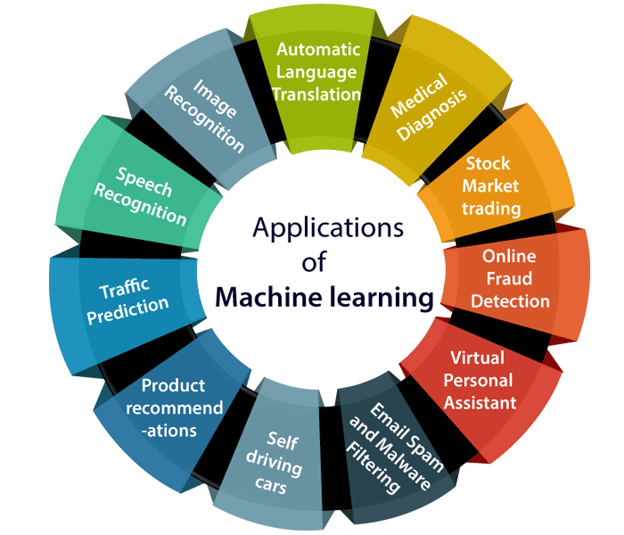
\includegraphics[width=0.5\linewidth]{figures/machine-learning-applications.png}
    \caption{Few applications of machine learning.}
    \label{fig:machine_learning_applications}
\end{figure}

%% here was reached
% TODO rewrite this part
% https://www.ibm.com/blog/mlops-and-the-evolution-of-data-science/
\section{The Evolution of MLOps}
With the rise of machine learning, so did the need for efficient operations around it. This led to the evolution of \ac{MLOps}
\ac{MLOps} is an engineering practice that aims at making the process of deploying machine learning models more efficient, reliable, and maintainable.
It uses \ac{CI/CD} and machine learning models to rationalize the monitoring, deployment and maintenance of machine learning systems.

\subsection{Key Components of MLOps}

As the datasets to train machine learning models got bigger and more complex, the realization for the need of \ac{ML} life cycle grow, as the old techniques weere slow and difficult to scale.
Data scientists worked together with IT teams to create and develop an assembly line for each step of training machine learning models.
In this chapter we will discuss few steps of michine learning life cycle that are crucial for \ac{MLOps} process.
\begin{itemize}
\item \textbf{Data Collection}: Gathering and refining relevant data set from different sources to prepare it for modeling is one of the key components of ML life cycle.
\item \textbf{Building and training}: This is the step  where models are created and trained using data, that were prepared in the previous step. It involves selecting appropriate algorithms and preprocessing the data.
\end{itemize}
And more as shown in \autoref{fig:machine_learning_lifecycle}.
\begin{figure}[htbp]
    \centering
    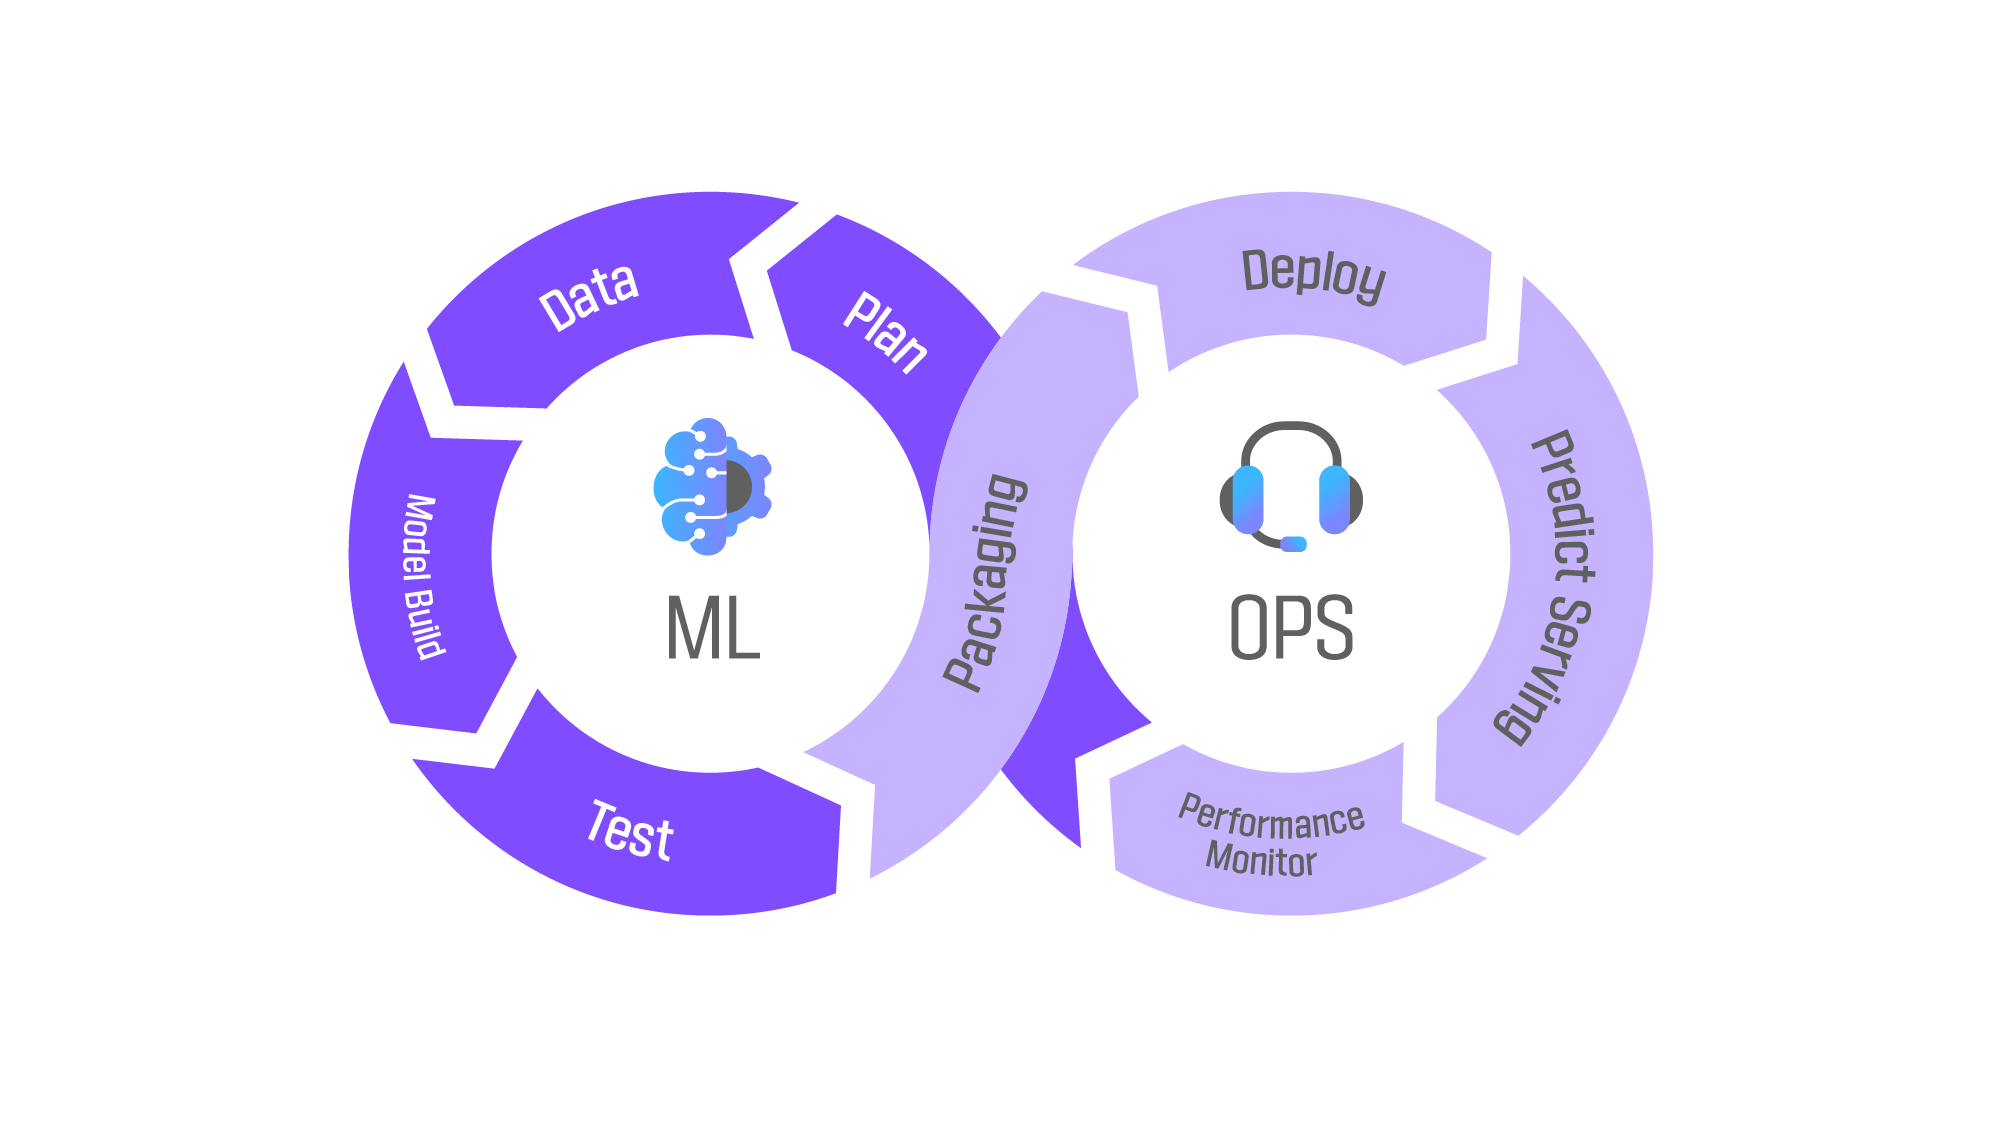
\includegraphics[width=0.78\linewidth]{figures/machine-learning-life-cycle.png}
    \caption{machine learning life cycle.}
    \label{fig:machine_learning_lifecycle}
\end{figure}

\subsection{Comparing MLOps and DevOps}

DevOps is a method which aims at bringing together software development and operations, it shortens the system's development life cycle and provides a continu delivery to a high software quality. 
\newline
\ac{MLOps} does, however, borrow from the DevOps principles of a rapid, continuous approach to writing and updating applications, in that they both have a code-validate-deploy loop. But the \ac{MLOps} life cycle contains additional steps, that are necessary for building and training the machine learning model as shown in \autoref{fig:DevOps_To_MLOPs}.
The aim in both cases is to take the project to production more efficiently with faster fixes, faster releases and ultimately, a higher quality product that boosts customer satisfaction, whether that’s software or machine learning models.
\begin{figure}[htbp]
    \centering
    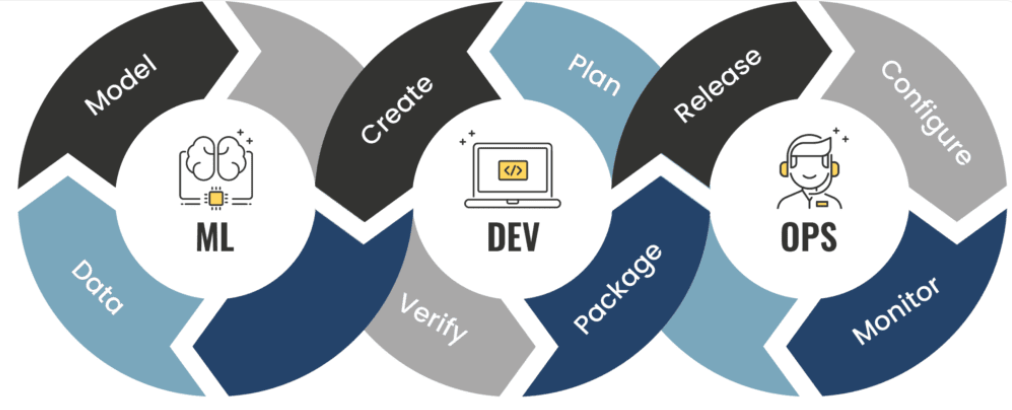
\includegraphics[width=0.78\linewidth]{figures/DevOps-To_MLOps.png}
    \caption{The transition from DevOps to MLOps life cycle.}
    \label{fig:DevOps_To_MLOPs}
\end{figure}
\newline
In this thesis, we delve into these aspects, aiming to bridge the gap between local ML implementation and successful code execution in production systems. Let us embark on this journey toward efficient \ac{MLOps} practices.
\chapter{The Gap: WHy Does It Exists}\label{chapter:gap}

Before diving into the details of bridging the gap between local code development
and cloud execution in \ac{MLOps}, it is essential to understand how the gap exists in the first place.
In this chapter, I will explore a brief explanation of why there is a gap between the two environments.

\section{Why the Gap Exists}
There is a notable distinction between running code locally on a developer's machine and deploying it to a cloud server for execution. This disparity can pose certain challenges in terms of infrastructure, environment, configuration and more, which can make it challenging to ensure seamless functionality across both environments.
\newline 
I would like to take this opportunity to examine a few of the reasons that have been presented. It is important to consider these reasons in a fair and impartial way:
\begin{itemize}
    \item Local development environments often have different configurations, dependencies, and resources than cloud environments. This can lead to inconsistencies and incompatibilities when deploying code to the cloud.
    \item Cloud environments often have different security, compliance, and scalability requirements than local environments. This can lead to additional complexity and overhead when deploying code to the cloud.
    \item Cloud environments often have different monitoring, logging, and debugging tools than local environments. This can make it difficult to diagnose and resolve issues that arise in the cloud.
\end{itemize}
In the coming chapters, I will discuss different approaches to overcoming these difficulties and how they
can be implemented in practice and put a spurt in the development and debugging
process on the cloud.



\chapter{Bridging the Gap}\label{chapter:solutions}

In the previous chapters, I explored the history of machine learning and provided a comprehensive overview of the most critical aspects of the \ac{MLOps} life cycle, and briefly discussed the reasons for why the gap between running code locally on developer's machine and deploying it in a cloud-based environment for running.
\newline
This chapter aims to introduce strategies for overcoming this gap and its associated challanges. Integrating these strategies requires a comprehensive understanding of both the theoretical and practical aspects of cloud computing and local development environments. It is important to point out that each strategy outlined in this chapter is accompanied by a comprehensive explanation of how it works, and include code examples that demonstrate its practical application.
\section{Containerization}
In order to grasp the concept of containerization, it is essential to understand the concept of vertualization and the differences between various virtualization mechanisms.

\subsection{Virtualization}
Virtualization is the process of creating a virtual version or several virtual versions of a piece of computer or a sofware according to cambridge dictionary \cite{cambridge_dictionary}. It is the art of creating a virtual version of somthing that does not exists physically, appearing as though is does.
\newline
In computer science, virtualization refers to replicating a physical system or server and its components within a single machine, to mimic their functionality. Basically, it is about sharing capabilities of a single physical machine accross multiple users or virtual settings. This approach empowered cloud service providers to share their physical infrastructure capabilities to user more efficiently.

\subsection{Containers vs. Virtual Machines}
We can distinguish between two primary forms of virtualization \cite{CON_VMS, CON_VMS_Atlassien, CON_VMS_ENGINE_YARD}:
\begin{enumerate}
    \item \textbf{\ac{VMs}}: \ac{VMs} virtualize an entire machine down to the hardware layers. They mimic the behavior of the underlying physical hardware/computer - like CPU, Disks and Networking devices - using a hypervisor, thus creating several virtual machines. Each virtual machine runs its \ac{OS} required for the respective applications, libraries, and functions separately from the other \ac{VMs}. Different \ac{VMs} can be run on the same physical host. Virtual machines may also include a complementary software stack to run on the emulated hardware. These hardware and software packages combined produce a fully functional snapshot of a computational system. As shown in \autoref{fig:Virtual_Machine}
          \begin{figure}[htbp]
    \centering
    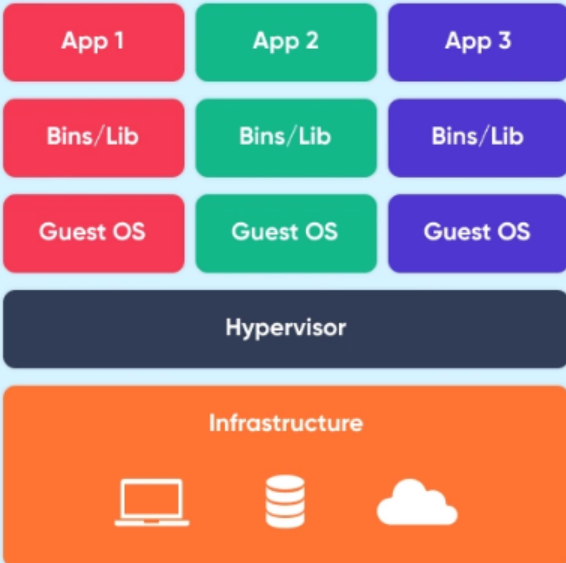
\includegraphics[width=0.4\linewidth]{figures/virtual_machine.png}
    \caption{Structure of vertual machines.}
    \label{fig:Virtual_Machine}
\end{figure}
          \newline
          \textbf{Advantages}
          \begin{itemize}
              \item \textbf{Complete Isolation}: \ac{VMs} operate in total isolation, effectivly wording as independent systems. this isolation ensures that these machine are protected from any harmful exploits, or interference from other \ac{VMs} sharing the same host. While it is still possible for a virtual machine to be vulnerable to some exlpoits, the contaminated virtual machine will not affect the neighboring \ac{VMs} due to this isolation, preventing any cross-contamination amoung virtual machines.
              \item \textbf{Dynamic Development}: \ac{VMs} offer more dynamic development environment. Starting from basic setup, virtual machine can be treated like individual computers. this adaptability enables the direct installation of software, enabling the hands-on development process. Additionally, virtual machines allow for the creating of images, capturing their configurations at any given time.
          \end{itemize}

          \textbf{Disadvantages}
          \begin{itemize}
              \item \textbf{Cost of Storage Space}: It is worth noting that virtual machine take up a lot of space, due to the fact that they virtualize the entire machine. This expansion can lead to potential disk storage issues as the virtual machines keep expanding. Therefor it is crucial to keep monitoring and managing the consumtion to ensure optimal performance and to avoid any disruption on the virtual machine.
              \item \textbf{Speed of Iteration}: Creating and maintaining a virtual machines can be a complex and time-consuming process, as it involves setting up an entire system stack. Modefiying a snapshot of a virtual machine can require significant efforts to rebuild and ensure its expected functionality.  
          \end{itemize}
    \item \textbf{Containers}: Containers take an alternative approach, by bunding the application with its necessary binaries, libraries and dependencies into a single package. Unlike traditional techniques, containers mimic the host operating system, giving each container the illusion of being isolated and that it is interactiting with its own virtual kernal, while the truth is, that all containers on host are sharing the same kernal. As demonstrated in \autoref{fig:Containers}. This shared kernal design alloes one \ac{OS} instance to run several isolated containers, making them lightweight and faster to boot compared to virtual machines. This efficiency is resource management and the accelerated application delivery highlights the advantages of containers over \ac{VMs}.
          \begin{figure}[htbp]
    \centering
    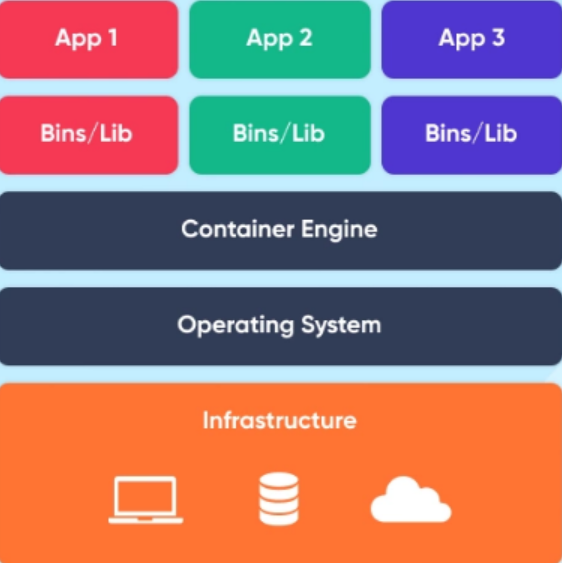
\includegraphics[width=0.445\linewidth]{figures/containers.png}
    \caption{General structure of containers.}
    \label{fig:Containers}
\end{figure}
          \newline
          \textbf{Advantages}
          \begin{itemize}
              \item \textbf{Speed of Iteration}: Due to the fact that containers are lightweight and include only the essential high-level software, as we saw earlier, they possess a remarkable capability for rapid development and iteration. Their basic design and focus on minimalism allow efficient modification capabilities.
              \item \textbf{Robust ecosystem}: Container runtime system offer developers access to pre-defined repositories. These repositories provide an extensive selection of popular software applications, such as databases and messaging systems, that are fast to restore and execute. This setup can help development teams to save time and focus on their core tasks.
          \end{itemize}

          \textbf{Disadvantages}
          \begin{itemize}
              \item \textbf{Shared host exploits}: Containers are built on a shared hardware infrastructure below the operating system layer. That means it is possible that an exploit in one container could break out of the container and affect the hardware that is shared with other containers. This poses a security risk when using one of these public images as they may contain exploits or be vulnerable to being hijacked by nefarious actors.
              % TODO add one more cons 
          \end{itemize}
\end{enumerate}
\subsection{Docker}
\subsection{Why Use Docker in Machine Learning}
\subsection{Example}

%% adding a new page to seperate this two sections (for now)
\newpage

\section{Hybrid Approaches}

\section{Cloud Execution}
\chapter{Evaluation}\label{chapter:evaluation}
\chapter{Conclusion}\label{chapter:conclusion}
% TODO: add more chapters here
%
\appendix{}

\microtypesetup{protrusion=false}

\addchap{Abbreviations}
\begin{acronym}
	\itemsep-.25\baselineskip
	\acro{TUM}[TUM]{Technical University of Munich}
	\acro{ML}[ML]{Machine Learning}
	\acro{AI}[AI]{Artificial Intelligence}
	\acro{MLOps}[MLOps]{Machine Learning Operations}
	\acro{NN}[NN]{Neural Network}
	\acro{CNN}[CNN]{Convolutional Neural Networks}
	\acro{CI/CD}[CI/CD]{Continuous Integration and Continuous Deployment}
	\acro{VMs}[VMs]{Virtual Machines}
	\acro{OS}[OS]{Operating System}
	\acro{cgroups}[cgroups]{Control Groups}
	% TODO: add acronyms
\end{acronym}

\listoffigures{}
\listoftables{}
\microtypesetup{protrusion=true}
\printbibliography{}

\end{document}
